\chapter{KPTimes: des mots-clés éditeurs pour la génération de mots-clés}\label{chap:kptimes}

Dans le chapitre~\ref{chap:framework}, nous avons recensé les principaux jeux de données exploités pour la production de mots-clés.
Ces jeux de données contiennent en moyenne \num{1000} documents, à l'exception de KP20k; cette quantité n'est pas suffisante pour entraîner des méthodes neuronales génératives qui requièrent des centaines de milliers de documents. \todo{une citation pour le nombre de doc d'entraînement des modèles neuronaux}
Ainsi, il manque un jeu de données similaire à KP20k (c'est-à-dire de grande taille) mais d'un domaine différent pour pouvoir évaluer la généralisation des méthodes de production automatique de mots-clés.
Nous avons retenu le domaine journalistique car de grandes quantités de documents sont facilement collectables et ils sont parfois annotés en mots-clés.
De plus, les mots-clés des documents scientifiques sont majoritairement annotés par les auteurs.
Cette annotation génère de nombreux biais que nous détaillerons au chapitre~\ref{chap:large-scale-eval}. En particulier, les effets de mode biaisent le choix des mots-clés, l'objectivité des annotateurs et la cohérence entre les annotateurs.

Pour pallier ces inconvénients, nous avons constitué le jeu de données KPTimes, composé d'articles journalistiques en anglais et suffisamment grand pour entraîner des méthodes neuronales. KPTimes documente le domaine, la provenance et les auteurs de chaque document grâce à des métadonnées riches, contrairement à KP20k dont l'origine des documents est incertaine, et dont les différents domaines ne sont pas explicités. L'annotation en mots-clés a suivi un processus rigoureux qui garantit leur qualité et la cohérence de l'annotation. 

Dans ce chapitre, nous présentons d'abord le processus de collecte de KPTimes. Nous présentons ensuite ses statistiques en le comparant aux jeux de données comparables en termes de genre (articles journalistiques) et en termes de taille (KP20k). Enfin, nous analyserons les performances des méthodes de production automatique de mots-clés sur KPTimes ainsi que les capacités de généralisation des méthodes neuronales sur KPTimes et KP20k.

\section{Constitution du jeu de données}

Dans cette section nous présentons d'abord le processus de constitution du jeu de données KPTimes: la collecte des données et le filtrage des documents.
Ensuite, nous décrivons ce jeu de données en exposant ses statistiques. Un exemple de document extrait de KPTimes est présenté dans la figure~\ref{fig:ex_kptimes}.

% From https://latexcolor.com
%\definecolor{yellow}{rgb}{0.99, 0.76, 0.0} % goldenpoppy
%\definecolor{green}{rgb}{0.0, 0.62, 0.38} % shamrockgreen
%\definecolor{blue}{rgb}{0.13, 0.67, 0.8} % ballblue
%\definecolor{red}{rgb}{0.87, 0.36, 0.51} % blush
%\definecolor{orange}{rgb}{1.0, 0.43, 0.29} % outrageousorange

\begin{figure*}[!htbp]
    \centering
    \resizebox{0.98\textwidth}{!}{%
    \begin{tabular}{|p{1.05\textwidth}|}
    \textbf{\textcolor{color1}{Muslim} \textcolor{color5}{Women} in Hijab Break Barriers: \lq{}Take the Good With the Bad\rq{}}
    
    \vspace{0.5em}
    
    When Ginella Massa, a Toronto-based TV reporter, recently accepted a request to host an evening newscast, she was not planning or expecting to make history for wearing a hijab. She was just covering for a colleague who wanted to go to a hockey game. And that's how Ms.~Massa, who works at CityNews in Toronto, became the first Canadian woman to host a newscast from a large \textcolor{color3}{media} company while wearing the head scarf.
    [...]
    This new trend of inclusion occurs amid a more sinister one, as reported \textcolor{color4}{hate crimes} against \textcolor{color1}{Muslims} are on the rise in the United States and \textcolor{color2}{Canada}. The F.B.I. says that a surge in \textcolor{color4}{hate crimes} against \textcolor{color1}{Muslims} has led to an overall increase in \textcolor{color4}{hate crimes} in the United States; \textcolor{color1}{Muslims} have borne the brunt of the increase with 257 recorded attacks.
    [...]
    In \textcolor{color2}{Canada}, where Ms.~Massa has lived since she was a year old, the number of reported \textcolor{color4}{hate crimes} has dropped slightly overall, but the number of recorded attacks against \textcolor{color1}{Muslims} has grown: 99 attacks were reported in 2014, according to an analysis by the \textcolor{color3}{news} site Global \textcolor{color3}{News} of data from Statistics \textcolor{color2}{Canada}, a government agency.
    [...]

    \vspace{0.5em}
    
    \textbf{Mots-clés de référénce:} US; Islam; Fashion; \textcolor{color1}{Muslim}~Veiling; \textcolor{color5}{Women} and Girls; (\textcolor{color3}{News media}, journalism); \textcolor{color4}{Hate~crime}; \textcolor{color2}{Canada}
    \end{tabular}%
    %lieu
    %general subject
    %geenral subject
    %general subject
    %general subject
    %general subject
    %general subject
    %lieu
    }
    \caption{Document extrait de KPTimes (id: \texttt{ny0296216}). Les mots apparaissant dans le document sont colorés.}
    \label{fig:ex_kptimes}
\end{figure*}

\subsection{Sélection des sources de données}

Nous avons constitué ce jeu de données de manière automatique à partir d'articles journalistiques extraits du site \url{nytimes.com}.
Ce site a été choisi car les métadonnées des articles contiennent des mots-clés annotés de manière semi-automatique par les éditeurs du journal.
Les éditeurs se trouvent à la fin de la chaîne de production des articles et sont chargés des dernières vérifications avant publication: choisir le titre, les mots-clés et mettre en page le journal.

% Particularité des éditeurs
L'annotation éditeur se fait de manière semi-automatique. Pour cela un système d'indexation contrôlée propose un ensemble de mots-clés aux éditeurs.
Ceux-ci peuvent alors réviser l'ensemble, c'est-à-dire ajouter ou supprimer des mots-clés, qu'ils fassent partie du vocabulaire contrôlée ou non.\footnote{\url{https://media.lac-group.com/blog/rules-based-tagging-metadata}}
Ces révisions sont ensuite prises en compte par le système d'indexation contrôlée pour les prochaines indexations.
Les mots-clés du système d'indexation contrôlée relèvent de cinq catégories~\cite{sandhaus_new_2008}:
\begin{itemize}
    \item lieux, p. ex. \foreign{Brooklyn},
    \item personnes, p. ex. \foreign{Bernie Sanders},
    \item titres d'oeuvres, p. ex. \foreign{Snow White and the Seven Dwarfs},
    \item structures et entreprises, p. ex. \foreign{Pfizer Inc},
    \item sujets généraux, p. ex. \foreign{Skateboarding}.
\end{itemize}
% Différence avec les variantes de semeval-2010
Ainsi ce processus d'annotation est mixte: il combine les avantages de l'annotation contrôlée (cohérence) grâce à l'algorithme, et libre (exhaustivité) grâce à la révision des éditeurs.

Dans le but d'observer les capacités de généralisation des méthodes à d'autres types d'annotation en mots-clés, nous constituons un second ensemble d'articles à partir du site \url{japantimes.co.jp} qui sera intégré à l'ensemble de test de KPTimes. Les articles du Japan Times contiennent aussi des mots-clés dans les métadonnées.
%
Depuis 2013, l'édition du week-end du Japan Times inclut l'\foreign{International New York Times}, ce qui laisse penser que ces deux journaux ont une ligne éditoriale similaire et qu'ils traitent de sujets similaires.
%
Nous décrivons séparément ces deux sous-ensembles d'articles extraits du New York Times et du Japan Times et le jeu de données KPTimes dans son ensemble.

Après filtrage (voir section~\ref{ssec:kptimes_filter}), les documents sont séparés en ensembles de test, entraînement et validation.
L'assignation des documents à ces ensembles se fait de manière aléatoire, en vérifiant que le ratio de mots-clés présents, la longueur et la distribution dans les différentes catégories soient comparables.
L'ensemble de test est composé par les documents du New York Times et du Japan Times en quantités égales.
Nous mettons à disposition les documents au format \texttt{jsonl}.\footnote{\url{https://github.com/ygorg/KPTimes}}

%Il existe un corpus, \say{The New York Times Annotated Corpus}~\cite{sandhaus_new_2008} constitué lui aussi d'articles jorunalistiques du New York Times décrivant les différents champs présents dans les métadonnées des pages web aspirées.
%Notamment le processus d'annotation des champs \say{Descriptors} qui sont agrégés dans la balise \say{keyword} des pages web aspirées.
%
%Ce processus est décrit dans la Figure~\ref{fig:kptimes_annotation_process}.
% A faire en tikz ? et en largeur
\iffalse
\begin{figure}
    \centering
    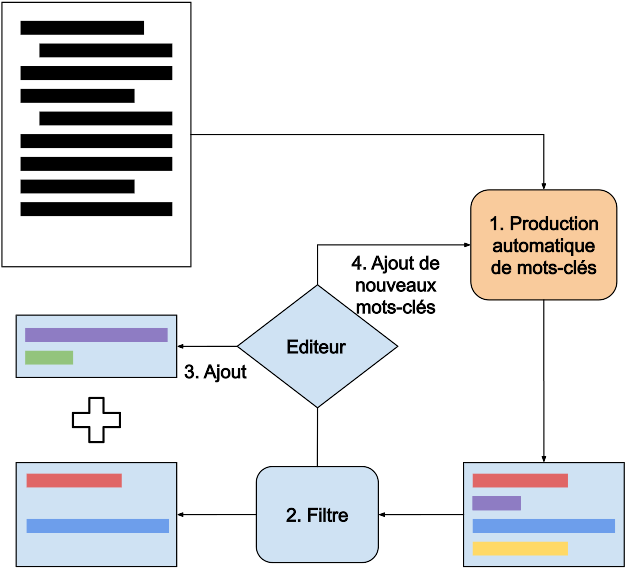
\includegraphics[width=20em]{figures/KPTimes_editor_annotation.png}
    \caption{Processus d'annotation par les éditeurs du New York Times.}
    \label{fig:kptimes_annotation_process}
\end{figure}
\fi

\subsection{Collecte des données}

La collecte des données concerne deux journaux en anglais: le New York Times et le Japan Times.

%\paragraph{NYTimes}
Les articles du New York Times ont été collectés de manière automatique par moissonnage. Les articles disponibles gratuitement sont répertoriés par date sur une page web\footnote{\url{https://spiderbites.nytimes.com/}}, nous en avons extrait les URL des articles de 2006 à 2017.

\begin{figure}[!htbp]
    \begin{subfigure}{.48\textwidth}
        \centering
        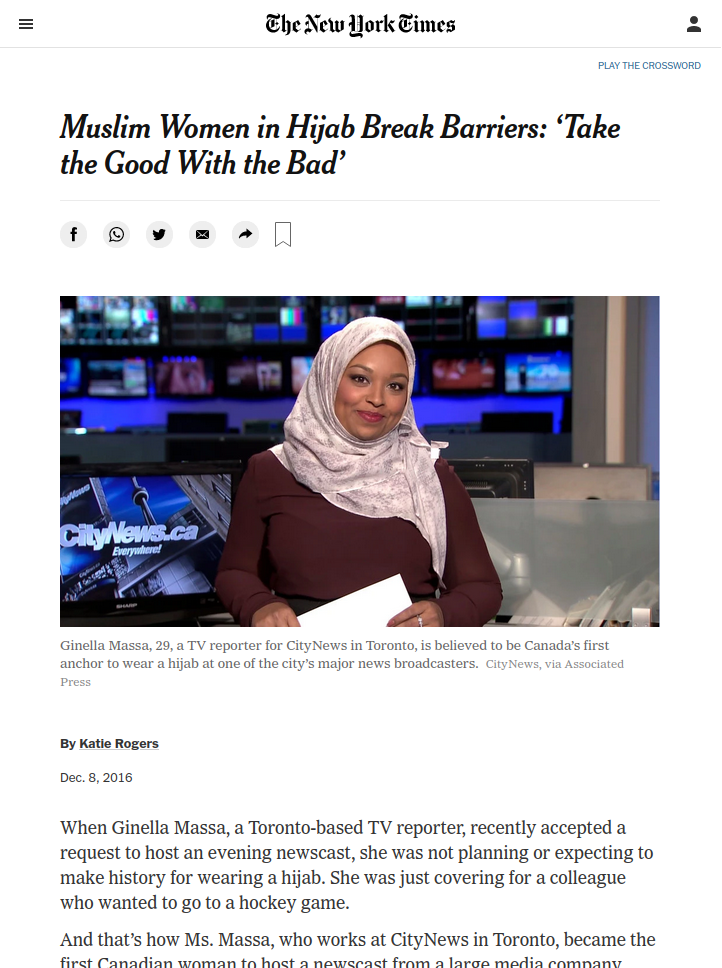
\includegraphics[scale=0.28]{4_kptimes/figures/image_kptimes.png}
        \caption{Capture d'écran d'un article sur le site du New York Times.}
        \label{fig:img_kptimes}
    \end{subfigure}%
    \hfill
    \begin{subfigure}{.48\textwidth}
\begin{minted}[
frame=lines,framesep=2mm,
baselinestretch=0.9,fontsize=\scriptsize
]{html}
<html><body>
<title>Muslim Women in Hijab Break Barriers:
‘Take the Good With the Bad’ - The New York
Times</title>
<meta name="description" content="
    Even as reports of hate crimes against 
    Muslims rise in America and Canada, 
    hijabis are appearing in makeup ads, 
    beauty pageants and news anchor chairs.
    ">
<meta name="byl" content="By Katie Rogers">
<meta name="news_keywords" content="
    Muslim Veiling,,Hate crime, Women and 
    Girls,Canada,US,Islam,Fashion,
    News media;journalism,">
<meta name="CG" content="world">
<meta name="SCG" content="americas">
<meta name="pdate" content="20161208">
<meta name="url" content="
    https://www.nytimes.com/2016/12/08/
    world/americas/hijab-muslim-women.html">
...
</head><body>
When Ginella Massa, a Toronto-based ...
</body></html>
\end{minted}
    \caption{Code source d'un article du site du New York Times.}
    \label{fig:meta_kptimes}
\end{subfigure}%
    
    
    \iffalse
    \begin{subfigure}{.48\textwidth}
        \centering
        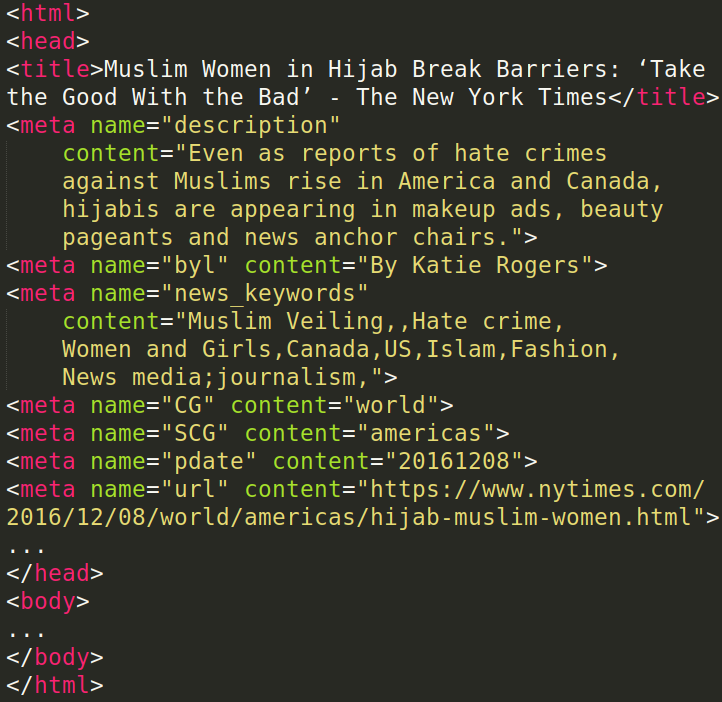
\includegraphics[scale=0.27]{4_kptimes/figures/html_kptimes.png}
        \caption{Code source d'un article du site du New York Times.}
        \label{fig:meta_kptimes}
    \end{subfigure}%
    \fi
    \caption{Version web et \texttt{html} de l'article \texttt{ny0296216} du jeu de données KPTimes.}
    \label{fig:kptimes_ex_img}
\end{figure}

Cela représente \num{296974} articles au format \texttt{html} composés du titre, de la \foreign{headline} (résumé en une ligne), du corps de l'article et des métadonnées. Parmi les métadonnées (voir figure~\ref{fig:meta_kptimes}), nous conservons la date de publication, la catégorie de l'article, l'auteur et les mots-clés.
La mise en page de l'article (décrite par le format \texttt{html}) encode des annotations telles que la séparation en paragraphes, les ancres de liens et la mise en forme matérielle (voir figure~\ref{fig:img_kptimes}).
Nous avons choisi de ne pas incorporer ces informations dans KPTimes mais nous indiquons l'URL de chaque document qui permet de reconstruire la collection et d'accéder aux documents \texttt{html} originaux.

Les articles du Japan Times sont au nombre de  \num{11057} et ont été collectés dans une période de 2008 à 2019 (dont \npercent{70} datent de 2019). Les métadonnées sont similaires à celles du New York Times: les articles sont séparés en catégories, sont associés à des mots-clés et contiennent une \foreign{headline}. 

\subsection{Filtrage des documents collectés}\label{ssec:kptimes_filter}

Un examen manuel des documents montre que certains articles sont redondants, trop longs ou trop courts. Nous décrivons ici le processus de filtrage de ces articles.

\paragraph{Redondance}
Deux articles sont des doublons s'ils partagent le même titre et le même texte, auquel cas nous n'en conservons qu'un. La suppression des doublons concerne \num{2233} articles. Les cas de doublons arrivent lorsque le même article est publié à deux dates différentes.

Deux types d'articles présentent aussi des similarités sans être des doublons: 
\begin{itemize}
    \item les articles récurrents, qui partagent un même contenu, tels que l'agenda des sorties ou les résultats du loto, et qui ne diffèrent que par des dates, des chiffres et autres informations ne modifiant pas les sujets abordés;
    \item les articles suivis, couvrant un même évènement dans le temps.
\end{itemize}
Ces deux types d'articles ont la particularité  de partager un  identifiant journalier (\foreign{slug}) et le même ensemble de mots-clés.
Par exemple, l'identifiant journalier des 464 articles présentant les résultats de la loterie est \say{lottery-numbers-for-new-york-new-jersey-and-connecticut}. Sur ces 464 articles 296 partagent le même ensemble de mots-clés: \foreign{Connecticut}, \foreign{Lotteries}, \foreign{New Jersey}, \foreign{New York State}.
Pour supprimer les articles similaires, nous les regroupons à l'aide de leur identifiant journalier, puis nous supprimons les groupes d'articles où plus de \npercent{70} des documents ont le même ensemble de mots-clés, soit \num{2533} articles. 
Nous avons fixé ce ratio à \npercent{70} pour inclure certains articles similaires dont le contenu diffère significativement malgré une majorité de mots-clés identiques.
Ce ratio permet par exemple de conserver une série d'articles couvrant des manifestations en Thaïlande qui partagent le même identifiant journalier \say{thailand-protest} et des mots-clés similaire (Bangkok, Thailand, Yingluck Shinawatra, Thaksin Shinawatra) mais qui ont chacun un sujet différent.


\paragraph{Longueur}
Nous souhaitons homogénéiser la taille des documents en écartant les documents trop longs qui nécessitent beaucoup de mémoire pour être traités avec des méthodes neuronales, et les documents trop courts qui contiennent peu d'informations.
Les articles trop longs sont identifiés à l'aide de l'écart interquartile utilisé pour identifier les valeurs extrêmes en termes de longueur de mots. Pour la limite haute, nous choisissons 10 fois l'écart interquartile.
Nous supprimons ainsi 77 articles dont la longueur est supérieure à \num{8163} (le plus long fait \num{31893} mots). Ces articles sont des reportages ou des transcriptions de discours, ils diffèrent donc des articles journalistiques.
Les documents ayant une longueur inférieure à 100 mots sont aussi supprimés, soit \num{9326} documents. Ces documents correspondent pour les $2/3$ à des brèves de la catégorie sport.


Les documents du Japan Times sont filtrés de la même manière que les articles provenant du New York Times pour la redondance. En termes de longueur seuls les documents supérieurs à 1 fois l'écart interquartile sont supprimés, les documents du Japan Times étant en moyenne plus courts que ceux du New York Times.


%\paragraph{JPTimes}
%\subsection{Données de test pour la généralisation}

%Dans le but d'observer les capacités de généralisation des modèles, nous constituons un jeu de donnée à partir du site \url{japantimes.co.jp}. Les articles de journal en ligne contient des mots-clés affichés dans l'article et dans ses métadonnées.
%De ce site, \num{11057} articles sont collectés et seront inclus dans ensemble de test.
%Ces documents sont filtrés de la même manière que les articles provenant du New York Times pour la redondance, en terme de longueur seuls les documents supérieur à 1 fois l'écart interquartile sont supprimés, les documents étant plus court que ceux du New York Times en moyenne.
% Se restreindre à une seule source de données, assure l'uniformité et la cohérence de l'annotation, manquante dans les autres jeux de données d'articles journalistiques, mais cela rend aussi les modèles entraînés dépendant à la source et nuis à la généralisation.
% Pour observer les capacités de généralisation des modèles, nous rassemblons une source de données secondaires. Nous collections les pages HTML du Japan Times et les traitons de la manière décrite plus haut. 10\,K nouveaux articles composent le jeu de données Japan Times.



\subsection{Description statistique}

Le tableau~\ref{tab:kptimes_stats} présente les statistiques des ensembles de test de KPTimes (qui rassemble NYTimes et JPTimes), ainsi qu'à des fins de comparaison, les jeux de données d'articles journalistiques KPCrowd et DUC-2001 et le jeu de données de notices scientifiques de grande taille KP20k. Nous détaillons et commentons ci-après ces statistiques.


\begin{table}[htbp!]
\centering
\resizebox{0.98\textwidth}{!}{
    \begin{tabular}{lcrrrr
    S[table-format=2.1,table-number-alignment=right] S[table-format=2.1,table-number-alignment=right] S[table-format=5.0,table-number-alignment=right] S[table-format=1.1,table-number-alignment=right]}
    
     & & \multicolumn{3}{c}{Corpus} & 
    \multicolumn{3}{c}{Document} & 
    \multicolumn{2}{c}{Mots-clés} \\
    \cmidrule(lr){3-5} \cmidrule(lr){6-8} \cmidrule(lr){9-10} \\[-1.2em]
    
    \textbf{Corpus} &
    \textbf{Ann.} &
    \textbf{\#Entr.} &
    \textbf{\#Val.} &
    \textbf{\#Test} &

    \textbf{\#mots} &
    \textbf{\#mc} &
    \textbf{\%abs} &
    
    \textbf{\#uniq.} &
    \textbf{\#ass.} \\

    \cmidrule(lr){1-2} \cmidrule(lr){3-5} \cmidrule(lr){6-8} \cmidrule(lr){9-10}

    \textbf{KPTimes}       & $E$ &260\,K&20\,K &  20\,K & 738 &   5.0 & 38.4 & 20535 & 5.0 \\ % 1.03
    \quad \textbf{JPTimes} & $E$ &    - &     - &  10\,K & 570 &   5.0 & 24.2 &  8611 & 5.9 \\ % 0.86
    \quad \textbf{NYTimes} & $E$ &260\,K&20\,K &  10\,K & 905 &   5.0 & 52.5 & 13387 & 3.8 \\ % 1.34
    \addlinespace
    KPCrowd       & $L$ &  450 &     - &     50 & 465 &  46.2 &  8.1 &  1937 & 1.2 \\ % 38.74
    DUC-2001      & $L$ &    - &     - &    308 & 847 &   8.1 &  3.1 &  1800 & 1.4 \\ % 5.84
    \addlinespace
    KP20k         & $A$ &530\,K& 20\,K &  20\,K & 176 &   5.3 & 42.4 & 53489 & 2.0 \\ % 2.67

    \bottomrule

    \end{tabular}
}
\caption{Comparaison des statistiques de KPTimes et ses sous-ensembles de test JPTimes et NYTimes avec les jeux de données d'articles journalistiques et KP20k. Les mots-clés de référence sont annotés par des \underline{$L$}ecteurs, des \underline{$E$}diteurs ou des \underline{$A$}uteurs. La table présente le nombre de documents dans les corpus d'entraînement (\#Entr.), de validation (\#Val.) et de test (\#Test) ainsi que le nombre moyen de mots (\#mots), de mots-clés (\#mc) et le ratio de mots-clés absents (\%abs) par document. Les colonnes \#uniq. et \#ass. montrent le nombre de mots-clés uniques et le nombre moyen d'assignation d'un mot-clé.}
\label{tab:kptimes_stats}
\end{table}

% Nombre de documents
\paragraph{Taille du jeu de données}
KP20k contient deux fois plus de documents d'entraînement que KPTimes, 530\,K contre 260\,K, mais le même nombre de documents de test et de validation (20\,K). Malgré sa taille moins importante par rapport à KP20k, KPTimes permet néanmoins l'entraînement de méthodes neuronales.
Les tailles des ensembles de test de KPCrowd et DUC-2001 (centaine de documents) ne sont pas dans le même ordre de grandeur que KPTimes et KP20k (de l'ordre de dizaines de milliers).
%KPCrowd et DUC-2001 contiennent moins de documents de test que KPTimes et KP20k.
DUC-2001 ne propose pas de documents d'entraînement.


% Longueur des documents
%\paragraph{Longueur des documents}
%Les documents journalistiques de KPTimes sont similaires en termes de nombre de mots avec KPCrowd et DUC-2001. Le sous-ensemble de test JPTimes est comparable à celui de KPCrowd et NYTimes à celui de DUC-2001. L'utilisation conjointe de ces deux sources de données permet donc de couvrir un large spectre d'articles journalistiques. % y a des articles long et court (là on couvre les longueur des 2 dataset existant en 1 dataset)
% A vérifier section 3 genre du document Les articles journalistiques sont en moyenne plus longs que les notices scientifiques de KP20k

% Nombre de mots-clés (pas très intéressant, permet de souligner que c'est une annotation différente, mais ce sera dit juste après)
\paragraph{Nombre de mots-clés}

Le jeu de données KPTimes est assez proche de KP20k en termes de nombre de mots-clés malgré les genres différents de documents qu'ils rassemblent et les différentes procédures d'annotation. Ils ont respectivement 5,3 et 5,0 mots-clés par document en moyenne. Les jeux de données journalistiques KPCrowd et DUC-2001 annotés par des lecteurs contiennent plus de mots-clés en moyenne que KPTimes et KP20k, respectivement, 46,2 et 8,1.

% mots-clés absents
\paragraph{Mots-clés absents}

KPCrowd et DUC-2001 ont moins de \npercent{10} de mots-clés absents, cela est lié à leur annotation lecteur qui privilégie les mots-clés présents dans le document à l'inverse de l'annotation éditeur de KPTimes.
L'ensemble de test de KPTimes est similaire à KP20k en termes de mots-clés absents, respectivement \npercent{38.4} et \npercent{42.4}. Les ensembles d'apprentissage de KPTimes (documents du NYTimes) et KP20k ont un taux de mots-clés absents du même ordre de grandeur, respectivement \npercent{52.5} et \npercent{42.4}.  
%Le taux de mot-clés absents est important dans ces deux jeux de données puisqu'il représente plus d'un tiers des mots-clés. 

% Annotation plus cohérente
\paragraph{Qualité d'annotation}
KPTimes diffère des autres jeux de données par son annotation. L'annotation éditeur de KPTimes est semi-automatique, la proposition des mots-clés par un système automatique permet d'associer à un concept le même mot-clé de manière plus cohérente qu'une annotation libre lecteur ou auteur.
%
% Figure
Cette différence d'annotation est mise en lumière par le pourcentage de mots-clés en fonction du nombre d'assignations par document. 
La figure~\ref{fig:kptimes_kw_distrib} donne ce pourcentage pour les ensembles de test des trois jeux de données KPCrowd, KP20k et KPTimes annotés respectivement par des lecteurs, des auteurs et des éditeurs.
Par exemple, pour KP20k, \npercent{80} des mots-clés ne sont assignés qu'à un document, \npercent{10} des mots-clés à deux documents, \npercent{3} des mots-clés à trois documents, etc.
Entre l'annotation lecteur et l'annotation éditeur, le nombre de mots-clés assigné une seule fois baisse de \npercent{22,6}. Ce chiffre révèle la cohérence de l'annotation aidée d'un vocabulaire contrôlé par rapport à une annotation libre où le même concept peut être associé à différentes variantes de mots-clés (voir figure~\ref{tab:variants}).

\usepgfplotslibrary{fillbetween}

\begin{figure}[ht!]
    \centering
    %\resizebox{0.7\textwidth}{!}{%
    \begin{tikzpicture}
	    \begin{axis}[height=5cm,
	                 width=8.5cm,
	                 grid style={dashed,gray!30},
	                 ymajorgrids,
                     xlabel={Nombre d'assignements},
                     ylabel={\% de MC de référence},
                     every node near coord/.append style={font=\footnotesize},
                     ybar=0pt,
                     %ybar,
                     bar width=9pt,
                     ymin=0,
                     ymax=100,
                     xmin=0.3,
                     xmax=5.7,
                     tick align=inside,
                     legend entries={KPCrowd (lecteurs), KP20k (auteurs), KPTimes (éditeurs)},
                     legend cell align={left},
                     legend style={font=\small},
                     ]

            % 500N-KPCrowd Test
            \addplot [draw=green!80!black, fill=green!10, pattern=north east lines] coordinates {
                (1, 86.8)
                (2, 9.0)
                (3, 2.9)
                (4, 1.0)
                (5, 0.1)
            };
            
            % DUC-2001 Test
            %\addplot [draw=green, fill=green!15] coordinates {
            %    (1, 82.1)
            %    (2, 9.6)
            %    (3, 4.2)
            %    (4, 1.5)
            %    (5, 0.8)
            %};

            % KP20k Test
            \addplot [draw=blue, fill=blue!15] coordinates {
                (1, 79.4)
                (2, 10.2)
                (3, 3.5)
                (4, 1.8)
                (5, 1.1)
            };
            
            % KPTimes
            \addplot [draw=red, fill=red!15, pattern=dots, nodes near coords, point meta=explicit symbolic] coordinates {
                (1, 64.2)
                (2, 12.3)
                (3, 5.6)
                (4, 3.2)
                (5, 2.1)
            };
            
            \node (A1) at (axis cs:0.73,86.8) {};
            \node (A2) at (axis cs:1.26,64.4) {};
            \draw[->,>=latex,red!80!black] (A1) to[bend left] node (sum) [midway, right, font=\small] {\textcolor{red!80!black}{-22,6}} (A2);
            
            \node (B1) at (axis cs:1.73,9) {};
            \node (B2) at (axis cs:2.26,12.4) {};
            \draw[->,>=latex,green!60!black] (B1) to[bend left] node (sum) [midway, above, font=\small] {\textcolor{green!60!black}{+3,3}} (B2);
            
            \node (C1) at (axis cs:2.73,2.9) {};
            \node (C2) at (axis cs:3.26,6.1) {};
            \draw[->,>=latex,green!60!black] (C1) to[bend left] node (sum) [midway, above, font=\small] {\textcolor{green!60!black}{+2.7}} (C2);
            
            \node (D1) at (axis cs:3.73,1.0) {};
            \node (D2) at (axis cs:4.26,3.0) {};
            \draw[->,>=latex,green!60!black] (D1) to[bend left] node (sum) [midway, above, font=\small] {\textcolor{green!60!black}{+2,2}} (D2);
            
            \node (E1) at (axis cs:4.73,0.1) {};
            \node (E2) at (axis cs:5.26,2.0) {};
            \draw[->,>=latex,green!60!black] (E1) to[bend left] node (sum) [midway, above, font=\small] {\textcolor{green!60!black}{+2,0}} (E2);

        \end{axis}
    \end{tikzpicture}%
    %}
    \vspace*{-1em}
    \caption{Distributions de l'assignement des mots-clés de référence pour les mots-clés assignés à 5 documents ou moins.}
    \label{fig:kptimes_kw_distrib}
    \vspace*{-1em}
\end{figure}


% KP20K Train
%\addplot [draw=blue, fill=blue!15] coordinates {
%    (1, 69.7)
%    (2, 13.1)
%    (3, 5.0)
%    (4, 2.7)
%    (5, 1.7)
%};

%TermITH-Eval
%\addplot [draw=red, fill=red!15, nodes near coords, point meta=explicit symbolic] coordinates {
%    (1, 68.2) [\textcolor{red!80!black}{~~~~~-11.2}]
%    (2, 16.4) [\textcolor{green!60!black}{+6.2}]
%    (3, 5.4) [\textcolor{green!60!black}{+1.9}]
%    (4, 3.4) [\textcolor{green!60!black}{+1.6}]
%    (5, 1.9) [\textcolor{green!60!black}{+0.8}]
%};

% DUC-2001 Test
%\addplot [draw=green, fill=green!15] coordinates {
%    (1, 82.1)
%    (2, 9.6)
%    (3, 4.2)
%    (4, 1.5)
%    (5, 0.8)
%};

% KDD
%\addplot [draw=blue, fill=blue!15] coordinates {
%    (1, 78.6)
%    (2, 11.5)
%    (3, 3.6)
%    (4, 1.6)
%    (5, 1.1)
%};

Le tableau~\ref{tab:kptimes_comp_ass_kw} précise le nombre moyen d'assignations d'un mot-clé à un document pour les ensembles de test, d'apprentissage et de validation des jeux de données KP20k et KPTimes.
L'augmentation du nombre moyen d'assignations d'un mot-clé dans l'ensemble d'entraînement par rapport à l'ensemble de test s'explique par le nombre plus important des documents.
Un modèle entraîné sur KP20k apprend $\simeq$\num{650000} mots-clés différents alors qu'un modèle entraîné sur KPTimes en apprend seulement $\simeq$\num{100000}.
L'espace de recherche plus restreint de KPTimes facilite donc l'apprentissage de modèles supervisés.
La cohérence dans l'annotation de KPTimes décrite plus haut fait qu'un même mot-clé est présenté en moyenne 13 fois au modèle pendant l'apprentissage, contre 4 fois pour KP20k.
Cette meilleure représentativité des mots-clés de KPTimes par rapport à KP20k nous porte à croire qu'elle devrait influencer favorablement les performances des modèles appris. 

\begin{table}[htbp!]
\centering
    \begin{tabular}{l S[table-format=2.1,table-number-alignment=right] S[table-format=6.0,table-number-alignment=right] S[table-format=2.1,table-number-alignment=right] S[table-format=6.0,table-number-alignment=right]}
    & \multicolumn{2}{c}{\textbf{KP20k}} & \multicolumn{2}{c}{\textbf{KPTimes}} \\
    \cmidrule(lr){2-3} \cmidrule(lr){4-5} \\[-1.5em]
    & \small{\#ass.} &   \small{\#uniq.} &  \small{\#ass.} &   \small{\#uniq.} \\
    \midrule
    Test  & 2,0 &  53489 &   5.0 &  20535 \\ % NYTimes + JPTimes
    Val.  & 2,0 &  52975 &   3.9 &  13269 \\ % NYTimes
    Entr. & 4,3 & 648697 &  13.1 & 101748 \\ % NYTimes
    \bottomrule
    \end{tabular}
\caption{Comparaison du nombre de mots-clés total et du nombre moyen d'assignation d'un mot-clé entre les ensembles de test, de validation et d'entraînement de KPTimes et KP20k.}
\label{tab:kptimes_comp_ass_kw}
\end{table}

\paragraph{Catégories des documents}
Les articles journalistiques de KPTimes sont classés en plusieurs catégories et sous-catégories thématiques (par exemple \foreign{Science}, \foreign{Région de NY} et \foreign{Sports}).
Ces catégories peuvent servir à entraîner des modèles spécialisés ou à analyser plus finement les performances des méthodes de production automatique de mots-clés.
Le tableau~\ref{tab:kptimes_categories} présente la distribution des articles dans chacune des catégories des sous-ensembles de test NYTimes et JPTimes.
Les catégories de ces deux sous-ensembles ne sont pas alignées. En effet, il n'y a pas de lien direct entre les deux ensembles de catégories bien que la catégorie \foreign{Sports} se retrouve dans les sous-catégories de JPTimes.
Cette absence d'alignement s'explique par la différence de granularité des deux ensembles de catégories thématiques, NYTimes regroupe les articles par thématiques alors que JPTimes les regroupe plutôt par aire géographique. Seule la catégorie \say{Business} est comparable en termes de nombre de documents entre ces deux sous-ensembles.

\begin{table}[htbp!]
    \centering
    \begin{subtable}{0.4\textwidth}
        \centering
        \resizebox{\textwidth}{!}{
        \begin{tabular}{rS[table-format=2.1,table-number-alignment=center]}
        \toprule
            \textbf{Catégorie}   & \textbf{\% d'articles} \\
            \midrule
            Sports       & 24.0 \\
            Monde        & 19.7 \\
            Business     & 19.1 \\
            Région de NY & 15.3 \\
            U.S.         & 15.3 \\
            Technologie  & 3.4 \\
            Science      & 3.0 \\
            Politique    & 0.1 \\
        \bottomrule
        \end{tabular}
        }
        \caption{NYTimes}
        \label{tab:nytimes_categories}
    \end{subtable}
    %
    \begin{subtable}{0.4\textwidth}
        \centering
        \resizebox{\textwidth}{!}{
        \begin{tabular}{rS[table-format=2.1,table-number-alignment=center]}
        \toprule
            \textbf{Catégorie}   & \textbf{\% d'articles} \\
            \midrule
            National   & 35.1 \\
            Monde      & 28.1 \\
            Business   & 23.0 \\
            Asie-Pacifique & 12.3 \\
            Reference  & 1.5 \\
            General    & 0.1 \\
        \bottomrule
        \end{tabular}
        }
        \caption{JPTimes}
        \label{tab:jptimes_categories}
    \end{subtable}
    \caption{Distribution des articles du jeu de données KPTimes par catégories dans l'ensemble de test.}
    \label{tab:kptimes_categories}
\end{table}

%conclusion
%Cette étude comparative entre KPTimes et les jeux de données KPCrowd, DUC-2001 et KP20k montre que l'annotation en mots-clés est plus cohérente pour KPTimes que pour les autres jeux de données.
%que KPTimes rassemble assez de documents pour entraîner les modèles neuronaux et 
%Nous faisons donc l'hypothèse que les modèles neuronaux de production de mots-clés appris sur KPTimes seront plus performants que ceux appris sur KP20k, ce que nous étudierons dans la section suivante.



%Le vocabulaire de mots-clés est plus petit que les autres jeux de données. En effet il y a moins d'hapax que dans KP20k par exemple ou des jeux de données annotés par des lecteurs.
%L'homogénéité dans les données est un indicateur fort qui met en avant la qualité des données que l'on a collecté. Cela vient en réponse aux problématiques des autres jeux de données.

\section{Performances du jeu de données}\label{sec:kptimes_valid}

%\iffalse
\definecolor{color1}{rgb}{0.9699521567340649, 0.4569882390259858, 0.36385324448493633}
\definecolor{color2}{rgb}{0.903599057664843, 0.511987276335809, 0.19588350060161624}
\definecolor{color3}{rgb}{0.8087954113106306, 0.5634700050056693, 0.19502642696727285}
\definecolor{color4}{rgb}{0.7350228985632719, 0.5952719904750953, 0.1944419133847522}
\definecolor{color5}{rgb}{0.6666319352625271, 0.6197366714155128, 0.19396267878823373}
\definecolor{color6}{rgb}{0.5920891529639701, 0.6418467016378244, 0.1935069134991043}
\definecolor{color8}{rgb}{0.3126890019504329, 0.6928754610296064, 0.1923704830330379}
\definecolor{color9}{rgb}{0.19783576093349015, 0.6955516966063037, 0.3995301037444499}
\definecolor{color10}{rgb}{0.20312757197899856, 0.6881249249803418, 0.5177618167447304}
\definecolor{color11}{rgb}{0.20703735729643508, 0.6824290013722435, 0.5885318893529169}
\definecolor{color13}{rgb}{0.21387918628643265, 0.6720135434784761, 0.693961140878689}
\definecolor{color14}{rgb}{0.21786710662428366, 0.6656671601322255, 0.7482809385065813}
\definecolor{color15}{rgb}{0.22335772267769388, 0.6565792317435265, 0.8171355503265633}
\definecolor{color16}{rgb}{0.23299120924703914, 0.639586552066035, 0.9260706093977744}
\definecolor{color17}{rgb}{0.4768773964929644, 0.5974418160509446, 0.9584992622400258}
\definecolor{color18}{rgb}{0.6423044349219739, 0.5497680051256467, 0.9582651433656727}
\definecolor{color19}{rgb}{0.774710828527837, 0.49133823414365724, 0.9580114121137316}
\definecolor{color20}{rgb}{0.9082572436765556, 0.40195790729656516, 0.9576909250290225}
\definecolor{color21}{rgb}{0.9603888539940703, 0.3814317878772117, 0.8683117650835491}
\definecolor{color22}{rgb}{0.9633321742064956, 0.40643825645731757, 0.7592537599568671}
\definecolor{color23}{rgb}{0.9656056642634557, 0.4245907603266889, 0.6579786740552919}
\fi


\definecolor{color1}{rgb}{1, 1, 1}
\definecolor{color2}{rgb}{1, 1, 1}
\definecolor{color3}{rgb}{1, 1, 1}
\definecolor{color4}{rgb}{1, 1, 1}
\definecolor{color5}{rgb}{1, 1, 1}
\definecolor{color6}{rgb}{1, 1, 1}
\definecolor{color8}{rgb}{1, 1, 1}
\definecolor{color9}{rgb}{1, 1, 1}
\definecolor{color10}{rgb}{1, 1, 1}
\definecolor{color11}{rgb}{1, 1, 1}
\definecolor{color13}{rgb}{1, 1, 1}
\definecolor{color14}{rgb}{1, 1, 1}
\definecolor{color15}{rgb}{1, 1, 1}
\definecolor{color16}{rgb}{1, 1, 1}
\definecolor{color17}{rgb}{1, 1, 1}
\definecolor{color18}{rgb}{1, 1, 1}
\definecolor{color19}{rgb}{1, 1, 1}
\definecolor{color20}{rgb}{1, 1, 1}
\definecolor{color21}{rgb}{1, 1, 1}
\definecolor{color22}{rgb}{1, 1, 1}
\definecolor{color23}{rgb}{1, 1, 1}


\begin{figure}
    \centering
    %\centerfloat
    %\resizebox{1\textwidth}{!}{%
    \begin{mdframed}[backgroundcolor=blue!2, font=\small]
    
    \textbf{\hl{color9}{Fertilization} in \hl{color18}{Flowers} Marked by \hl{color15}{Expert Precision}}

    \vspace{0.9em}

    \hl{color18}{Flower} \hl{color9}{fertilization} is a \hl{color10}{complex process} that requires a \hl{color11}{perfect union} between a \hl{color3}{single} \hl{color2}{ovule} {and} a \hl{color3}{single} \hl{color5}{pollen} \hl{color21}{tube}, which contains \hl{color17}{sperm}. Now a \hl{color6}{new} \hl{color23}{study} reports how \hl{color18}{flowers} are able to reproduce with such \hl{color15}{expert precision}. \hl{color19}{Researchers} report that the moment a \hl{color13}{gamete} \hl{color22}{fusion} \hl{color14}{event} occurs — that is, when the two \hl{color17}{sperm} cells from a \hl{color5}{pollen} \hl{color21}{tube} unite with the two female \hl{color13}{gametes} in the \hl{color2}{ovule} — all other \hl{color5}{pollen} \hl{color21}{tubes} are repelled, redirected toward other \hl{color2}{ovules}. “As soon as the \hl{color22}{fusion} is successful, this mechanism is triggered that tells all the other \hl{color5}{pollen} \hl{color21}{tubes} to go away,” said Mark Johnson , a molecular geneticist at Brown University {and} an author of the \hl{color23}{study}, which is reported in the journal \hl{color16}{Current} \hl{color8}{Biology}. It isn’t clear exactly what causes the redirecting, Dr. Johnson said. “I don’t know if there’s a physical block to more \hl{color5}{pollen} \hl{color21}{tubes} coming,” he said. “We don’t see any evidence for that.” Most likely, “some sort of molecule is triggered that repels the other \hl{color5}{pollen} \hl{color21}{tubes},” he said. For a \hl{color18}{flowering} \hl{color4}{plant} like Arabidopsis — the one the \hl{color19}{researchers} \hl{color23}{studied} — to be as successful as possible, \hl{color2}{ovules} should not go to waste. The repelling feature helps \hl{color18}{flowers} attain maximum \hl{color20}{reproductive} success. {And} it is probably why \hl{color18}{flowering} \hl{color4}{plants} have generally been more successful than other \hl{color4}{plants} in colonizing the earth, Dr. Johnson said. “They’re basically everywhere,” he said.

    \vspace{1.1em}

\textbf{Mots-clés de référence}: \hl{color18}{Flowers}~{and}~\hl{color4}{Plants}, \hl{color20}{Reproduction}~(\hl{color8}{Biological}), Science~{and}~Technology, \hl{color16}{Current}~\hl{color8}{Biology}

\textbf{FirstPhrases}: \hl{color9}{fertilization}, \hl{color18}{flowers}, \hl{color15}{expert~precision}~\hl{color18}{flower}~\hl{color9}{fertilization}, \hl{color10}{complex~process}, \hl{color11}{perfect~union}

\textbf{TfIdf}: \hl{color18}{flowering}~\hl{color4}{plant}, \hl{color18}{flowers}, \hl{color15}{expert~precision}~\hl{color18}{flower}~\hl{color9}{fertilization}, \hl{color3}{single}~\hl{color2}{ovule}, \hl{color3}{single}~\hl{color5}{pollen}~\hl{color21}{tube}

\textbf{MPRank}: \hl{color18}{flowers}, \hl{color3}{single}~\hl{color5}{pollen}~\hl{color21}{tube}, \hl{color3}{single}~\hl{color2}{ovule}, \hl{color17}{sperm}, \hl{color6}{new}~\hl{color23}{study}

\textbf{Kea}: \hl{color18}{flowers}, \hl{color15}{expert~precision}~\hl{color18}{flower}~\hl{color9}{fertilization}, \hl{color3}{single}~\hl{color2}{ovule}, \hl{color3}{single}~\hl{color5}{pollen}~\hl{color21}{tube}, \hl{color13}{gamete}~\hl{color22}{fusion}~\hl{color14}{event}

\textbf{CopySci}: \hl{color18}{flower}~\hl{color9}{fertilization}, \hl{color5}{pollen}~\hl{color21}{tube}, \hl{color9}{fertilization}, \hl{color15}{expert~precision}, \hl{color5}{pollen}

\textbf{CopyNews}: \hl{color18}{flowers}~{and}~\hl{color4}{plants}, science~{and}~technology, \hl{color19}{research}, \hl{color5}{pollen}, \hl{color9}{fertilization}

    \vspace{0.2em}

    
    \end{mdframed}%
    %}
    \caption{Exemple de document de l'ensemble de test du corpus KPTimes (id: {\small ny0110694})). Les mots composants termes-clés présent dans le document sont soulignés.}
    \label{fig:_}
\end{figure}

% transférabilité du modèle appris
% capacité de généralisation du modèle
% 3 volets: même genre - annotation diff, même genre - annotation similaire; diff genre - annotation diff
Dans cette section, nous présentons et comparons les performances de plusieurs méthodes de production de mots-clés pour, dans un premier temps, attester de la validité de KPTimes, et dans un second temps, étudier la généralisation des méthodes à différents genres de documents et types d'annotations.

Nous comparons tout d'abord les résultats obtenus sur les jeux de données d'articles journalistiques (du même genre que KPTimes) mais dont l'annotation en mots-clés diffère.
Ensuite, nous comparons les performances des méthodes sur les deux sous-ensembles de test de KPTimes: NYTimes et JPTimes.
Ces ensembles de test comportent des documents du même genre et une annotation en mots-clés similaire.
Enfin, nous analysons la capacité de généralisation de la méthode CopyRNN grâce à une évaluation croisée sur KPTimes et KP20k, dont le genre des documents et le type d'annotation en mots-clés diffèrent.

% méthode état de l'art CopyRNN cf chap 2 
Nous choisissons de comparer les méthodes suivantes (décrites dans les sections~\ref{sec:methode-en-chaine-de-traitement} et \ref{methodes-de-bout-en-bout}): FirstPhrases, \tfidf{}, MultipartiteRank, Kea et CopyRNN. Nous rappelons les principales différences: FirstPhrases utilise uniquement la position; \tfidf{} la fréquence et la spécificité à un document; Kea combine ces deux indicateurs de manière supervisée; MultipartiteRank utilise la centralité dans un graphe; CopyRNN est une méthode neuronale générative. Nous utiliserons \textbf{CopyNews} pour désigner la méthode CopyRNN entraînée sur les articles journalistiques de KPTimes, et \textbf{CopySci} pour désigner CopyRNN entraînée sur les articles scientifiques de KP20k. Les paramètres utilisés sont ceux décrits par \citet{meng_deep_2017}.
% méthode d'évaluation F10 et mAP cf chap 3
Les mots-clés produits automatiquement sont évalués grâce au protocole décrit dans la section~\ref{sec:framework_evaluation}.


\subsection{Comparaison aux jeux de données journalistiques}

\begin{table}[htbp!]
    \centering
\begin{tabular}{l c@{\hspace*{1mm}}c c@{\hspace*{1mm}}c c@{\hspace*{1mm}}c}
 & \multicolumn{2}{c}{\textbf{KPTimes}} & \multicolumn{2}{c}{\textbf{DUC-2001}} & \multicolumn{2}{c}{\textbf{KPCrowd}} \\
  \cmidrule(lr){2-3} \cmidrule(lr){4-5} \cmidrule(lr){6-7} \\[-1.5em]
&    \small{$\text{F}@10$} &   \small{\map} &     \small{$\text{F}@10$} &   \small{\map} &         \small{$\text{F}@10$} &   \small{\map} \\
\midrule
FirstPhrases  &    11,4 &  10,7 &     24,3 &  22,3 &    17,1 &  16,5 \\
\tfidf{}         &    12,4 &  12,8 &     23,0 &  21,6 &    16,9 &  15,8 \\
MPRank        &    14,0 &  13,3 &     25,3 &  \best{24,9} & \best{18,2} &  \best{17,0} \\
\addlinespace
Kea           &    13,8 &  14,1 & \best{26,2} &  24,5 & 17,3 &  16,7 \\
\addlinespace
CopyNews       & \best{31,9} & \best{38,7} & 10,5 &   \pad{0}7,2 & \pad{0}8,4 &   \pad{0}4,2 \\
\bottomrule
\end{tabular}

    \caption{Performances de différents modèles de production de mot-clés sur des jeux de données d'articles journalistiques.}
    \label{tab:kptimes_perf_news}
\end{table}
Le tableau~\ref{tab:kptimes_perf_news} compare les performances de différentes méthodes de production de mots-clés sur des jeux de données journalistiques: KPTimes, DUC-2001 et KPCrowd.
Les performances des méthodes extractives (FirstPhrases, \tfidf{} et MPRank) sont bien plus basses sur KPTimes que sur DUC-2001 et KPCrowd: 10 points de différence de \map{} entre KPTimes et DUC-2001. Cette grande différence s'explique par leurs proportions différentes de mots-clés absents: KPTimes en contient \npercent{38.4} et DUC-2001 \npercent{3.1}.
En effet, les méthodes extractives ne proposent que des mots-clés présents dans les documents, c'est-à-dire que \npercent{38.4} des mots-clés de KPTimes ne peuvent être retournés par ces méthodes.

Les performances de la méthode CopyNews (CopyRNN entraîné sur KPTimes) sont étonnamment faibles sur DUC-2001 et KPCrowd (respectivement \npercent{7} et \npercent{4} de \map{}) et sont bien inférieures aux performances des méthodes extractives.
Cette grande différence est liée aux mots-clés de référence utilisés pour l'évaluation: CopyNews est entraîné à reproduire les mots-clés éditeurs de KPTimes alors que les mots-clés de DUC-2001 et KPCrowd ont été annotés par des lecteurs. Les mots-clés de ces deux types d'annotation sont très différents, en effet, seulement \npercent{13} des mots-clés de DUC-2001 et \npercent{19} des mots-clés de KPCrowd apparaissent aussi dans KPTimes.\footnote{Ces statistiques ont été calculées sur les ensembles de test.}

\begin{figure}
    \centering
    %\centerfloat
    \resizebox{0.98\textwidth}{!}{%
    \begin{tabular}{|p{1.3\textwidth}|}
    
    The \textcolor{color4}{tuberculosis} \textcolor{color8}{rate} in \textcolor{color7}{U.S.} \textcolor{color6}{prisons} may be more than three times higher than on the outside, federal \textcolor{color2}{health} officials said Thursday, urging testing, isolation and other measures to curb TB behind bars.
    %Researchers with the Centers for Disease Control cited a survey in 29 states, where \textcolor{color6}{prisons} reported 31 \textcolor{color4}{tuberculosis} \textcolor{color1}{cases} per 100,000 inmates in 1984-85, compared with eight \textcolor{color1}{cases} per 100,000 reported among non-incarcerated adults in those states during the same period.
    %\say{In some large correctional systems, the incidence of TB has increased dramatically,} the \textcolor{color5}{CDC} said, noting that in New York state there were 106 TB \textcolor{color1}{cases} per 100,000 inmates in 1986 -- seven times more than the average of 15 \textcolor{color1}{cases} reported in 1976-78.
    [\ldots]
    In \textcolor{color2}{New Jersey}, inmates had a TB \textcolor{color8}{rate} of 110 per 100,000 in 1987, 11 times higher than the general \textcolor{color2}{New Jersey} population. In California, the \textcolor{color8}{rate} was nearly six times higher -- 80 per 100,000. \textcolor{color4}{Tuberculosis}, a contagious, bacterial lung disease, occurs in about 22,000 new \textcolor{color1}{cases} each year in the United States ; most can be cured with drug treatment.
    As many as 7 percent of Americans have latent TB \textcolor{color0}{infections}, and about 10 percent of them will someday develop a \textcolor{color1}{case} of \textcolor{color4}{tuberculosis} itself.
    \say{Persons at highest risk... are close contacts,} the \textcolor{color5}{CDC} said, noting that TB can pose particular problems in \textcolor{color6}{prisons}, where there is often overcrowding and \say{where the environment is often conducive to \textcolor{color9}{airborne transmission} of \textcolor{color0}{infection} among inmates, staff and visitors.}
    %The \textcolor{color5}{CDC}'s Advisory Committee for the Elimination of \textcolor{color4}{Tuberculosis} is recommending TB testing for most new \textcolor{color6}{prison} inmates and staff members -- with the possible exception of inmates just transferring through for less than a week.
    %The \textcolor{color5}{CDC} committee also recommends new tests at least once a year, rapid chest X-rays for TB-infected people showing symptoms, and isolation -- off the \textcolor{color6}{prison} property, if necessary -- for those with suspected or confirmed symptomatic TB \textcolor{color1}{cases}.
    [\ldots]
    The spread of \textcolor{color3}{AIDS-virus} \textcolor{color0}{infections} may play a part in the spread of TB in \textcolor{color6}{prisons}, the \textcolor{color5}{CDC} said.
    AIDS weakens the immune system, making patients susceptible to \textcolor{color0}{infections} other people might ward off, including \textcolor{color4}{tuberculosis}.
    AIDS tests should be offered to all inmates with known TB \textcolor{color0}{infections}, the \textcolor{color5}{CDC} report said.

    \vspace{0.9em}

    

    \vspace{1.1em}
    \textbf{CopyNews}: \textcolor{color4}{tuberculosis}, \textcolor{color2}{new~jersey}, us, medicine~and~\textcolor{color2}{health}, \textcolor{color6}{prisons} \\
    \textbf{Mots-clés de référence}: \textcolor{color4}{tuberculosis}~\textcolor{color8}{rate}, \textcolor{color7}{u.s}.~\textcolor{color6}{prisons}, \textcolor{color3}{aids-virus}~\textcolor{color0}{infections}, \textcolor{color9}{airborne transmission}, \textcolor{color4}{tuberculosis}~\textcolor{color1}{cases}, \textcolor{color5}{cdc}
    \vspace{0.2em}


    \end{tabular}%
    }
    \caption{Exemple de document de l'ensemble de test du corpus DUC-2001 (id: {\small AP890511-0126})).}
    \label{fig:ex_kptimes_duc}
\end{figure}


Pour tempérer ces faibles résultats nous présentons dans la figure~\ref{fig:ex_kptimes_duc} un document extrait de DUC-2001 ainsi que ses mots-clés de référence et ceux produits par CopyNews.
Même si aucun des mots-clés de CopyNews n'est commun à ceux de la référence, ces mots-clés sont (pour la plupart) pertinent et reflètent les spécificités de l'annotation éditeur.
Par rapport à la référence, les sujets principaux sont bien identifiés (la tuberculose et la prison), le lieu est aussi bien identifié (\say{us}) même s'il s'agit d'une variante du mot-clé de référence. Le modèle prédit aussi le mot-clé \say{\foreign{new jersey}} qui est mentionné dans l'article mais n'est pas pertinent dans ce contexte.
%
Le mot-clé généré \say{\foreign{medicine and health}} est intéressant car il est spécifique à l'annotation éditeur. Il décrit le sujet global du document et a plus vocation à catégoriser le document qu'à décrire un de ses sujets en particulier.
Le modèle n'identifie en revanche pas les concepts de \say{cdc} (\foreign{Centers for Disease Control}) qui est la source de cet article, de \say{aids-virus infection} qui facilite la transmission de la tuberculose et de \say{\foreign{airborne transmission}} qui décrit la méthode de propagation du virus.
Ainsi, les mots-clés générés par le modèle, malgré leur faible correspondance aux mots-clés de référence, sont cohérents avec l'annotation éditeur qui identifie le lieu, les concepts principaux et les acteurs (individus, entreprises, etc.).


%Nous pouvons tirer la conclusion que CopyRNN n'est pas performant car n'arrive pas a reproduire une référence auteur (qui n'a jamais été vue dans l'ensemble d'entraînement) ni à extraire les mots-clés présents, ou alors que la comparaison de ces 

\subsection{Généralisation des méthodes neuronales}
\label{sub:kptimes_generalisation}
% étude qualitative ??

Nous présentons les performances des méthodes de production de mots-clés sur KPTimes et ses deux sous-ensembles de test, NYTimes et JPTimes dans le tableau~\ref{tab:kptimes_perf_split}.
Les méthodes extractives ont des performances plus élevées sur JPTimes que sur NYTimes: la F@10 de Kea est de 11,0 sur NYTimes contre 16,6 sur JPTimes.
Cette différence s'explique par le fait que JPTimes contient moins de mots-clés absents (\npercent{24,2}) que NYTimes (\npercent{52,5}).
Là encore, le taux de mots-clés absents  pénalise les méthodes exclusivement extractives.
Le modèle CopyNews entraîné sur les documents du NYTimes, est moins performant sur JPTimes, le score de \map{} est divisé par deux. Ces constatations montrent combien le modèle est dépendant de la référence sur laquelle il a été entraîné et c'est d'autant plus vrai pour les mots-clés absents. 
%En effet seuls \num{1463} mots-clés sont communs a JPTimes et NYTimes, 

\begin{table}[htbp!]
    \centering
    %\resizebox{\textwidth}{!}{
\begin{tabular}{l c@{\hspace*{1mm}}c|c@{\hspace*{1mm}}c c@{\hspace*{1mm}}c}
 & \multicolumn{2}{c}{\tiny{(NYT $+$ JPT)}}
 & \multicolumn{2}{c}{\multirow{2}{*}[-0.35em]{\textbf{NYTimes}}} & \multicolumn{2}{c}{\multirow{2}{*}[-0.35em]{\textbf{JPTimes}}} \\
 %[-0.6em]
 & \multicolumn{2}{c}{\textbf{KPTimes}} \\
 %& \multicolumn{2}{c}{\textbf{NYTimes}} & \multicolumn{2}{c}{\textbf{JPTimes}}\\
  \cmidrule(lr){2-3} \cmidrule(lr){4-5} \cmidrule(lr){6-7} \\[-1.5em]
&    \small{$\text{F}@10$} &   \small{\map} &   \small{$\text{F}@10$} &   \small{\map} &   \small{$\text{F}@10$} &   \small{\map} \\
\midrule
FirstPhrases  & 11,4 &  10,7 & \pad{0}9,2 & \pad{0}8,4 & 13,5 & 13,1 \\
\tfidf{}         & 12,4 &  12,8 & \pad{0}9,6 & \pad{0}9,4 & 15,1 & 16,2 \\
MPRank        & 14,0 &  13,3 & 11,2 & 10,1 & 16,8 & 16,5 \\
\addlinespace
Kea           & 13,8 &  14,1 & 11,0 & 10,8 & 16,6 & 17,5 \\
\addlinespace
CopyNews       & \best{31,9} &  \best{38,7} & \best{39,3} & \best{50,9} & \best{24,6} & \best{26,5} \\
\bottomrule
\end{tabular}
    %}
    \caption{Performances de différents modèles de production de mot-clés sur KPTimes et ses sous-ensembles de test.}
    \label{tab:kptimes_perf_split}
\end{table}

Le tableau~\ref{tab:kptimes_perf_generalisation} présente les performances de CopyNews et CopySci testées de manière croisée sur KPTimes et KP20k. 
Les performances hors situation de généralisation, c'est-à-dire avec CopyNews testé sur KPTimes et CopySci testé sur KP20k, sont plus élevées pour CopyNews que pour CopySci.
Cette différence de performance s'explique par la plus grande cohérence des mots-clés de KPTimes.
En situation de généralisation par contre, CopySci est plus performant que CopyNews. Les performances, par rapport à une évaluation non croisée, sont divisées par $\simeq5$ pour CopyNews et $\simeq2$ pour CopySci. Ainsi CopySci généralise donc mieux que CopyNews.
Ce résultat est étonnant étant donné les performances plus élevées de CopyNews évalué sur KPTimes.
Pour étudier plus finement cette différence de performances en situation de généralisation, nous nous intéressons au nombre de mots-clés générés par ces modèles.

\begin{table}[htbp!]
    \centering
    %\resizebox{\textwidth}{!}{
\begin{tabular}{l c@{\hspace*{1mm}}c c@{\hspace*{1mm}}c}
 & \multicolumn{2}{c}{\textbf{KPTimes}} & \multicolumn{2}{c}{\textbf{KP20k}} \\
 \cmidrule(lr){2-3} \cmidrule(lr){4-5} \\[-1.5em]
 &    \small{$\text{F}@10$} &   \small{\map} &  \small{$\text{F}@10$} &   \small{\map} \\
\midrule
CopyNews &\best{31,9}&\best{38,7}&\pad{0}6,6 & \pad{0}5,1 \\
CopySci  &    14,9 &  15,2 &\best{25,5}&\best{28,9}\\
\bottomrule
\end{tabular}
    %}
    \caption{Performances de généralisation du modèle CopyRNN entraîné sur KPTimes et KP20k.}
    \label{tab:kptimes_perf_generalisation}
\end{table}

Le tableau~\ref{tab:ratio_prsabs_transfer} présente le pourcentage de mots-clés présents et de mots-clés absents produits par les modèles CopyNews et CopySci sur KPTimes et KP20k. Le pourcentage de mots-clés absents produits automatiquement par le modèle CopyNews (\npercent{38.8}) est très proche de celui de la référence pour KPTimes (\npercent{38.4}). 
Le pourcentage de mots-clés absents produits automatiquement par le modèle CopySci (\npercent{8.0}) est très éloigné de celui de la référence pour KP20k (\npercent{42.4}).
Ces résultats montrent de nouveau la difficulté du modèle CopyRNN à reproduire l'annotation auteur, moins cohérente que l'annotation éditeur.
Ils montrent aussi que le modèle CopyRNN possède la capacité de générer un grand nombre de mots-clés absents, ce que nous ne pouvions savoir sans le jeu de données KPTimes et son annotation éditeur.
Nous remarquons que le pourcentage de mots-clés présents et absents produits par un modèle reste similaire en situation de généralisation, c'est-à-dire lorsque l'ensemble de test n'appartient pas au jeu de données utilisé pour l'entraînement.
Dans cette situation de généralisation, le modèle CopySci sur KPTimes obtient de meilleurs résultats que CopyNews sur KP20k. 
CopySci produit presque exclusivement des mots-clés présents (\npercent{94.6}) alors que CopyNews n'en produit qu'une courte majorité (\npercent{51.1}).
La généralisation pour la production de mots-clés absents est plus difficile que la production de mots-clés présents. 
Généraliser à un discours scientifique, lorsque l'apprentissage a été réalisé sur un discours généraliste, handicape la génération des mots-clés. 
Par exemple, le modèle CopyNews assigne le mot-clé \foreign{nyc} (\foreign{New York City}) à \num{2 137} documents de KP20k.
L'étude manuelle d'un échantillon de 30 documents montre que ce mot-clé n'a de rapport avec aucun de ces documents.
% Ce n'est pas le cas de scientifique à généraliste mettre des exemples de mots-clés générés dans les deux configurations

\iffalse
\begin{table}[htbp!]
    \centering
    \begin{tabular}{llSS}
        & & \textbf{KPTimes} &   \textbf{KP20k} \\
    \cmidrule(lr){3-4}
    %\cmidrule{1-4}
    \multirow{2}{*}{CopyNews}
        & Présent & 61.2 & 51.1 \\
        & Absent & 38.8 & 48.9 \\
        %& R & \best{11.73} & \best{2.62} \\
        %& M &  20.08 &  24.42 \\
        %& U & \best{7.02} & \best{21.85} \\
        \cmidrule(lr){1-2} \cmidrule(lr){3-4}
    \multirow{2}{*}{CopySci}
        & Présent &  94.9 &  92.0 \\
        & Absent &  5.1 &  8.0 \\
        %& R &   0.79 &   2.95 \\
        %& M &   1.27 &   2.87 \\
        %& U &   3.02 &   2.22 \\
    \bottomrule
    \end{tabular}
    \caption{Pourcentage de mots-clés présents et absents produit automatiquement par le modèle CopyRNN entraîné sur KPTimes (CopyNews) et KP20k (CopySci) et testé sur ces deux jeux de données.}
    \label{tab:ratio_prsabs_transfer}
\end{table}
\fi


\begin{table}[htbp!]
    \centering
    \begin{tabular}{lS@{\hspace*{1mm}}S S@{\hspace*{1mm}}S}
        & \multicolumn{2}{c}{\textbf{KPTimes}} & \multicolumn{2}{c}{\textbf{KP20k}} \\
    \cmidrule(lr){2-3} \cmidrule(lr){4-5} \\[-1.5em]
    & \small{Prs} & \small{Abs} & \small{Prs} & \small{Abs} \\
    \midrule
    %\cmidrule{1-4}
    {CopyNews}
        & 61.2 & 38.8 & 51.1 & 48.9 \\
    %\cmidrule(lr){1-2} \cmidrule(lr){3-4}
    {CopySci}
        & 94. & 5.1 &  92.0 & 8.0 \\
    \bottomrule
    \end{tabular}
    \caption{Pourcentage de mots-clés présents et absents produit automatiquement par le modèle CopyRNN entraîné sur KPTimes (CopyNews) et KP20k (CopySci) et testé sur ces deux jeux de données.}
    \label{tab:ratio_prsabs_transfer}
\end{table}

%CopyNews ne génère pas les mêmes types de mots-clés pour le jeu de données sur lequel il a été entraîné, KPTimes, et pour KP20k. Le nombre de mots-clés absent est bien plus élevé pour KP20k. Le modèle utilise le mécanisme de copie pour 72,91~\% de mots-clés pour KPTimes sur qui il a été entraîné, et seulement 53,73~\% pour KP20k.


%TODO: quel sont les résultats de CopyNews sur Inspec qui a des mots-clés indexeurs et donc plus qualitatifs que les autres datasets? Je m'attend a ce que CopyNews soit plus généralisable sur Inspec que CopySci. C'est-à-dire que CopyNews Inspec > CopySci Inspec. Car les annotations sont de meilleures qualités, ça devrait donc avoir un comportement similaire à JPTimes.
%TODO: Pourquoi CopySci est bon sur JPtimes et pas sur KPTimes. Est-ce que les bons mots-clés sur JPTimes de CopySci et CopyNews sont les mêmes ?? Si oui lesquels CopySci ne modélise pas bien? Si Non, qu'est-ce qui caractérise les MC modélisés par CopySci et CopyNews.

\section{Conclusion}

%4.1
Nous avons présenté notre contribution, le jeu de données KPTimes, composé d'articles journalistiques annotés de manière semi-supervisée par des éditeurs, et de taille suffisamment importante pour permettre l'entraînement de méthodes neuronales.
%4.2
Les documents ont été collectés de manière automatique sur les sites internet du New York Times et du Japan Times.
Les documents sont annotés de manière semi-automatique grâce à un système d'indexation contrôlée, vérifiée et enrichie par les éditeurs.
%4.1.4
Ce processus d'annotation résulte ainsi en une annotation beaucoup plus cohérente, facilitant l'apprentissage des méthodes neuronales.

%4.2.1
Nous avons ensuite mesuré les performances de plusieurs méthodes de production automatique de mots-clés sur KPTimes, puis nous les avons comparées à celles obtenues sur deux jeux de données journalistiques.
Nous avons constaté que les méthodes extractives étaient moins performantes sur KPTimes que sur les autres jeux de données (ce qui est lié au nombre plus important de mots-clés absents).
Nous avons aussi comparé les performances de méthodes neuronales entraînées sur KP20k et KPTimes, et avons trouvé que le modèle entraîné sur KPTimes est plus performant que celui entraîné sur KP20k.
%4.2.2
La création de KPTimes nous a permis de réaliser une première étude sur la capacité de généralisation des méthodes neuronales, c'est-à-dire lorsque l'entraînement et le test sont effectués sur des jeux de données différents.
Cette étude a montré la meilleure capacité de généralisation du modèle neuronal CopyRNN lorsqu'il est entraîné sur le jeu de données scientifiques KP20k que sur le jeu de données généralistes KPTimes.
%
Ce résultat est surprenant étant donné la meilleure qualité des mots-clés de KPTimes mais il est en fait lié à la faible capacité du modèle entraîné sur KP20k à produire des mots-clés absents.
En effet, il est moins risqué, pour avoir un rapport avec le document, de produire un mot-clé présent, limité au document, plutôt qu'un mot-clé absent.
Nous allons dans le chapitre suivant poursuivre nos expérimentations des différentes méthodes extractives et génératives en nous plaçant dans un cadre expérimental strict.



%sa référence contient \npercent{40} de mots-clés absent. Le modèle CopyRNN entraîné sur KPTimes dépend fortement de l'annotation éditeur et des documents journalistiques, en effet les performances sur des jeux de données comportant une référence différente ou des document d'un genre différent sont assez faibles. Le modèle CopyRNN entraîné sur KP20k (articles scientifiques) généralise mieux que le modèle entraîné sur KPTimes car il produit beaucoup plus (\npercent{95}) de mots-clés présent, qui peuvent être peu informatif mais qui lié au document.
%Dans un scénario de généralisation d'un modèle sur un autre genre de données, l'extraction de mots-clés semble le plus intéressant pour ne pas risquer de créer de faux mots-clés, des mots-clés qui n'auraient aucun rapport avec le document et qui dans un cadre d'indexation seraient contre-productifs.
%Évaluer automatiquement les performances de CopySci sur KPTimes, ou même sur DUC-2001 ne donne pas de bons résultats car l'évaluation automatique évalue si les mots-clés produits automatiquement correspondent à la référence, or un modèle qui produit des mots-clés éditeurs qui ne correspondent pas à une référence auteur (par exemple) ne pourra pas avoir de hautes performances, car on a appris au modèle à ne pas générer des mots-clés auteurs. L'évaluation dans un cadre de généralisation doit être effectuée manuellement pour évaluer le fait que les mots-clés produit soient liés au document plutôt que le fait qu'il correspondent à la référence.